\begin{figure}[t]
\centering
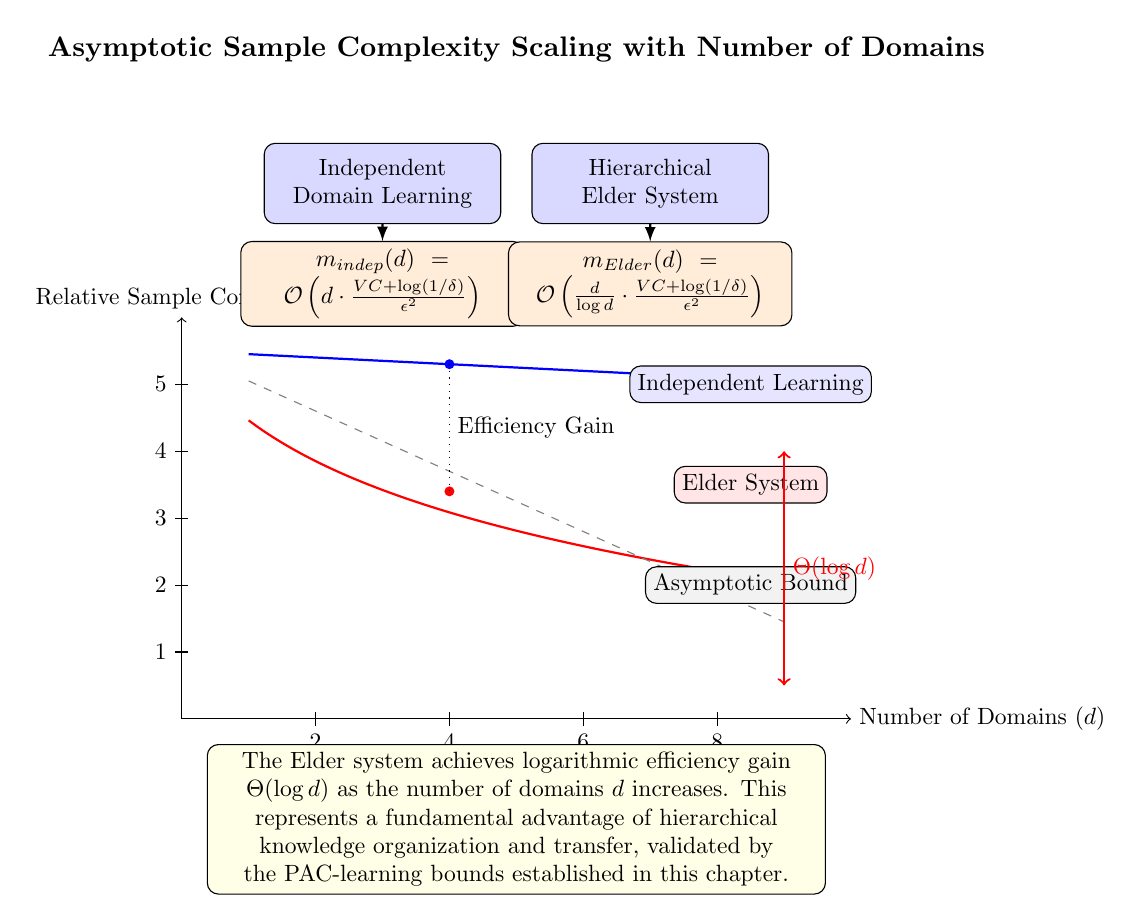
\begin{tikzpicture}[scale=0.85, transform shape]
    % Define styles
    \tikzset{
        system/.style={
            draw,
            fill=blue!15,
            rounded corners,
            minimum width=3.5cm,
            minimum height=1.2cm,
            text width=3.3cm,
            align=center
        },
        complexity/.style={
            draw,
            fill=orange!15,
            rounded corners,
            minimum width=4.2cm,
            minimum height=1cm,
            text width=4cm,
            align=center
        },
        arrow/.style={
            ->,
            thick,
            >=latex
        }
    }
    
    % Coordinate system for the main plot
    \draw[->] (0,0) -- (10,0) node[right] {Number of Domains ($d$)};
    \draw[->] (0,0) -- (0,6) node[above] {Relative Sample Complexity};
    
    % Sample points for independent learning
    \draw[domain=1:9, samples=50, smooth, variable=\x, blue, thick] plot ({\x}, {5.5 - 0.05*\x});
    
    % Sample points for Elder system
    \draw[domain=1:9, samples=50, smooth, variable=\x, red, thick] plot ({\x}, {5.5 - 1.5*ln(max(1.1,\x+1))});
    
    % Asymptotic bound
    \draw[domain=1:9, samples=50, smooth, variable=\x, gray, dashed] plot ({\x}, {5.5 - 0.45*\x});
    
    % System labels
    \node[draw, fill=blue!10, rounded corners, align=left] at (8.5,5) {Independent Learning};
    \node[draw, fill=red!10, rounded corners, align=left] at (8.5,3.5) {Elder System};
    \node[draw, fill=gray!10, rounded corners, align=left] at (8.5,2) {Asymptotic Bound};
    
    % System boxes
    \node[system] (indep) at (3,8) {Independent\\Domain Learning};
    \node[system] (elder) at (7,8) {Hierarchical\\Elder System};
    
    % Complexity boxes
    \node[complexity] (indep_complex) at (3,6.5) {$m_{indep}(d) = \mathcal{O}\left(d \cdot \frac{\text{VC} + \log(1/\delta)}{\epsilon^2}\right)$};
    \node[complexity] (elder_complex) at (7,6.5) {$m_{Elder}(d) = \mathcal{O}\left(\frac{d}{\log d} \cdot \frac{\text{VC} + \log(1/\delta)}{\epsilon^2}\right)$};
    
    % Connections
    \draw[arrow] (indep) -- (indep_complex);
    \draw[arrow] (elder) -- (elder_complex);
    
    % Logarithmic efficiency region
    \draw[<->, red, thick] (9,0.5) -- (9,4) node[midway, right] {$\Theta(\log d)$};
    
    % Reference markers on axes
    \foreach \x in {2,4,6,8}
        \draw (\x,0.1) -- (\x,-0.1) node[below] {$\x$};
    
    \foreach \y in {1,2,3,4,5}
        \draw (0.1,\y) -- (-0.1,\y) node[left] {$\y$};
    
    % Annotations for key points
    \node[circle, fill=blue, inner sep=1.5pt] at (4,5.3) {};
    \node[circle, fill=red, inner sep=1.5pt] at (4,3.4) {};
    \draw[dotted] (4,5.3) -- (4,3.4) node[midway, right] {Efficiency Gain};
    
    % Title
    \node[align=center, font=\bfseries, scale=1.2] at (5,10) {Asymptotic Sample Complexity Scaling with Number of Domains};
    
    % Explanation box
    \node[draw, rounded corners, fill=yellow!10, text width=9cm, align=center] at (5,-1.5) {
        The Elder system achieves logarithmic efficiency gain $\Theta(\log d)$ as the number of domains $d$ increases. This represents a fundamental advantage of hierarchical knowledge organization and transfer, validated by the PAC-learning bounds established in this chapter.
    };
    
\end{tikzpicture}
\caption{Asymptotic scaling of sample complexity with increasing number of domains. For independent domain learning (blue), sample complexity grows linearly with the number of domains. In contrast, the Elder system (red) exhibits sub-linear growth due to cross-domain knowledge transfer and universal principle extraction. The efficiency gain approaches $\Theta(\log d)$ asymptotically, demonstrating a fundamental advantage of the hierarchical Elder architecture that increases with scale. This logarithmic efficiency gain is a direct consequence of the PAC-learning bounds established in this chapter and validates the theoretical foundation of the Elder system.}
\label{fig:efficiency_scaling}
\end{figure}